\chapter{软件环境及设置}

该模版是基于CTeX社区发行的ctexbook模版,因此要使用该模版需要有CTeX环境。

与第一版稍有不同的时,由于该版提供了采用UTF-8编码的\XeTeX{}引擎的新版本和使用原有采用GBK编码的\LaTeX{}引擎的老版本,
因此,如果使用新版本,还需要参考本模版文件包中提供的ctex-xecjk-winfonts.def文件将自己系统中的
ctex-xecjk-winfonts.def文件进行修改,
该文件位于ctex目录下的$\backslash$tex$\backslash$latex$\backslash$ctex$\backslash$fontset目录下。
需要至少指定以下六种字体对应的字体文件:
\begin{verbatim}
\setCJKfamilyfont{zhsong}{SimSun}
\setCJKfamilyfont{zhhei}{SimHei}
\setCJKfamilyfont{zhkai}{KaiTi}
\setCJKfamilyfont{zhfs}{FangSong}
\setCJKfamilyfont{zhli}{LiSu}
\setCJKfamilyfont{zhyou}{YouYuan}

\newcommand*{\songti}{\CJKfamily{zhsong}} % 宋体
\newcommand*{\heiti}{\CJKfamily{zhhei}}   % 黑体
\newcommand*{\kaishu}{\CJKfamily{zhkai}}  % 楷书
\newcommand*{\fangsong}{\CJKfamily{zhfs}} % 仿宋
\newcommand*{\lishu}{\CJKfamily{zhli}}    % 隶书
\newcommand*{\youyuan}{\CJKfamily{zhyou}} % 幼圆
\end{verbatim}

其它字体可以自由指定,SimSun,SimHei这些指定字体的关键字可以直接用字体文件*.ttf 来代替,
也可以使用命令“fc-list”来具体查看系统中已安装的字体的名字,从而对应地填到上述命令中去。


\section{Microsoft Windows系统}

Windows系统下可以直接安装CTeX发行的软件包,该发行包只有32位版本,64位系统安装方法与32位略有不同。下面分别介绍。

\subsection{32位系统}

包括windows XP,Windows Server 2003,Vista, Windows Server 2008 和 Windows 7。

32位系统下安装比较简单,直接从www.ctex.org下载最新的安装包,当前最新版为2.9.0.152,
它包括CTeX环境,winEdt,MiKTeX,Ghostcript,几个部分,除CTeX环境外,
另外几个组件都可以选择安装,如可以用TeXLive替代MiKTeX,UltraEdit,gvim,Emacs替代winEdit等。
如果你不了解这几个软件,那么就默认安装选项即可。

安装完后,需要对\LaTeX 软件进行升级,如MiKTeX软件进行升级,升级的网络站点就选中科大的CTAN镜像站,
网址http://mirrors.ustc.edu.cn/CTAN,在教育网内速度还是比较快的,如图\ref{set1},\ref{set2},\ref{set3}所示。

\begin{figure}[th]
\centering
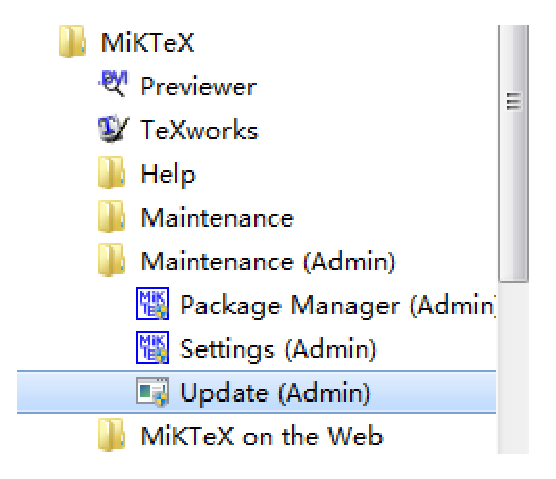
\includegraphics[scale=0.5]{./Pictures/set1.eps}\\
\caption{MiKTeX升级设置}
\label{set1}
\end{figure}

\begin{figure}[th]
\centering
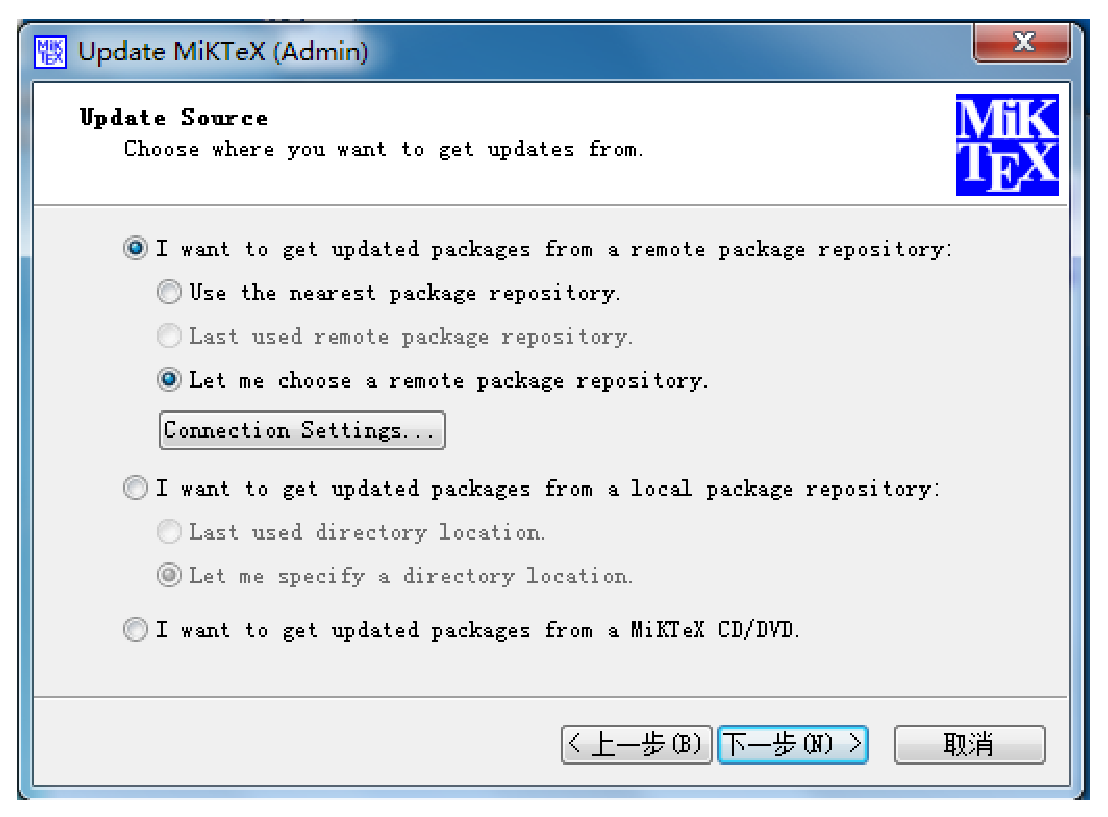
\includegraphics[scale=0.5]{./Pictures/set2.eps}\\
\caption{选择升级方式,如图中选择一个升级站点}
\label{set2}
\end{figure}

\begin{figure}[th]
\centering
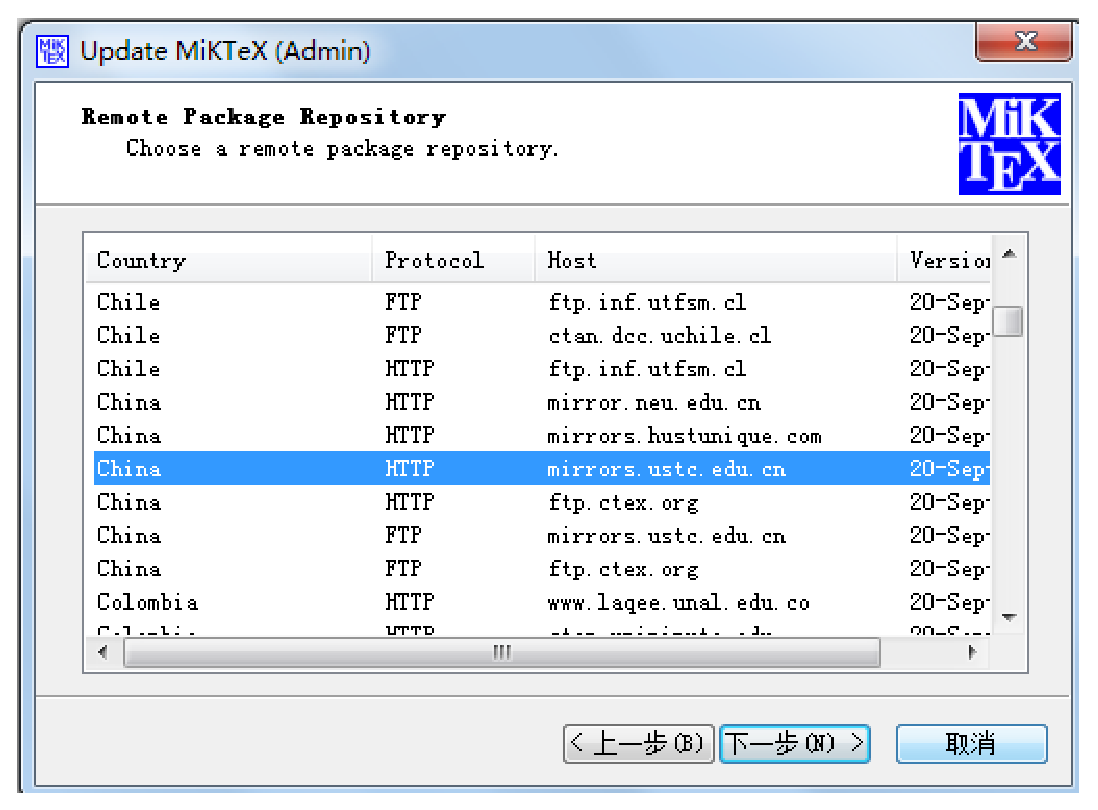
\includegraphics[scale=0.5]{./Pictures/set3.eps}\\
\caption{选择升级站点,以中科大镜像点为例}
\label{set3}
\end{figure}

之所以要把软件升级到最新是因为该模版使用了最新的hyperref包中添加的命令hidelinks。

\subsection{64位系统}

包括windows XP 64bit,Windows Server 2003 64bit,Vista 64bit,
Windows Server 2008 64bit,Windows 7 64bit 和 Windows Server 2008 R2。

安装CTeX安装包时,不要选择MiKTeX,其它软件任意,与32位一样。
安装完CTeX包后,去www.miktex.org网站下载MiKTeX的最新64位版,当前是2.9版,
安装后在设置页面中把CTeX的目录加到MiKTeX的Root目录中去,如图 \ref{setroot} 。
再如图 \ref{rffndb} 所示,刷新MiKTeX的目录数据库,就可以使用CTeX的环境了。

\begin{figure}[thp]
\centering
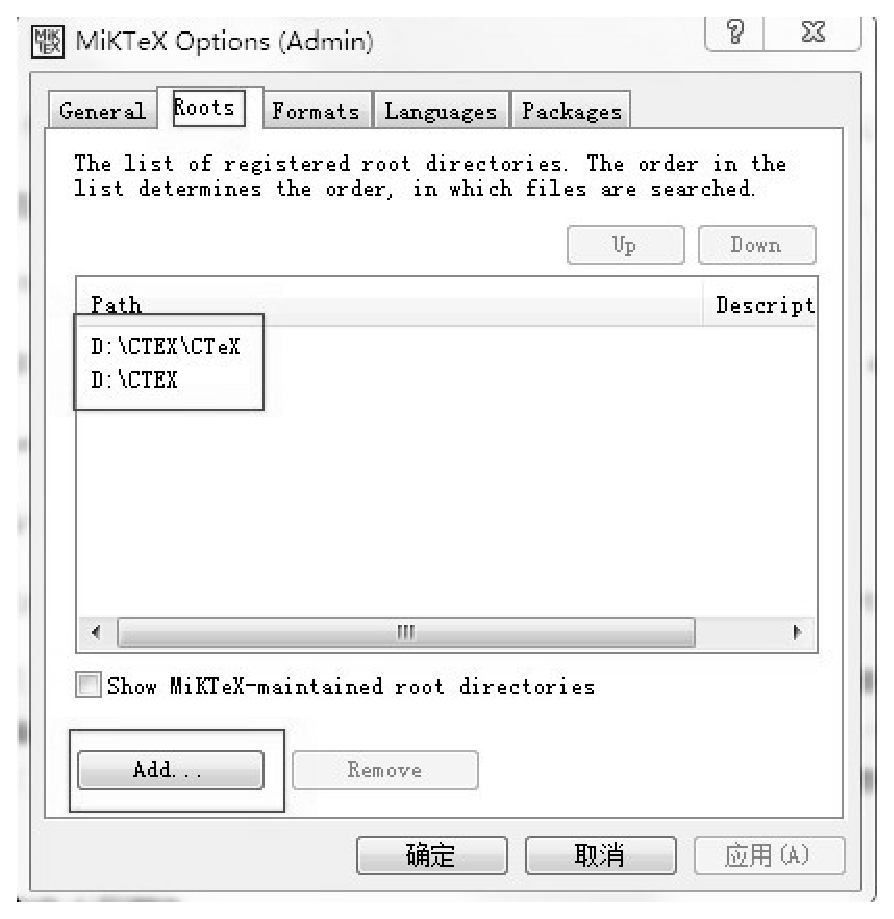
\includegraphics[scale=0.5]{./Pictures/setroot.eps}\\
\caption{设置MiKTeX软件的Root目录}
\label{setroot}
\end{figure}

\begin{figure}[th]
\centering
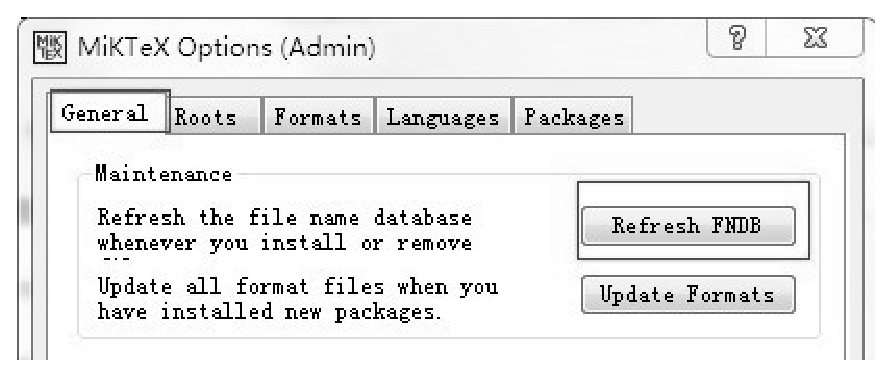
\includegraphics[scale=0.5]{./Pictures/rffndb.eps}\\
\caption{刷新MiKTeX的目录数据库}
\label{rffndb}
\end{figure}

与32位Windows系统相同,安装完后也需要把MiKTeX升级到最新。

\section{linux系统}

请自行选择\LaTeX 安装版本,然后把CTeX环境加入即可。我想用linux的应该都会这个吧。
本次版本使用的操作系统及软件环境是Debian 6和TeXLive2009。

请保证扩展包版本足够新。尤其是hyperref包,保证是2011年8月份后的版本。

\section{Mac系统}

请自行选择\LaTeX 安装版本,加入CTeX环境。同linux下。

\section{本模版所需要的扩展包}

\begin{enumerate}

\item{图形、表格类扩展包} graphicx,array,booktabs-de,caption,natbib,multirow

\item{字体类扩展包} times(\LaTeX{}引擎中用),fontspec(\XeTeX{}引擎中用)

\item{目录选项扩展包} tocbibind,tocloft,makeidx,hyperref

\item{数学公式扩展包} amsmath,amsthm,amsfonts,amssymb,bm

\end{enumerate}

\section{测试运行}

如果已经安装好了CTeX环境与\LaTeX 软件,那么,可以运行这个模版文件包里的makethesis.bat文件,
几秒钟到十几秒后,如果生成了一份叫做“论文模版示例.pdf”的文档,那么,恭喜,这个模版所需要的软件环境建立成功!
如果没有生成这一份文件,那么有可能你的软件环境没有配置正确,比如把\LaTeX 软件升级到最新,
这份模版所需要的扩展包没有被安装,请打开\LaTeX 软件自动升级功能,
保证\LaTeX 软件能够成功地连接到CTAN站点下载所需的扩展功能包。
